\documentclass{article}
\usepackage{graphicx} % Required for inserting images
\usepackage{minted} 

\title{Lista 1}
\author{Mateusz Kaczkowski}
\date{October 2025}

\begin{document}

\maketitle

Zadania na liście pierwszej polegały na napisaniu 3 algorytmów sortujących i ich wariantów zmodyfikowanych by tą samą metodą przerabiały większą ilość danych na raz, oraz przetestowaniu ich pod kątem ilości porównań i przypisań elementów tablicy. Jest to bardzo dobre przybliżenie rzeczywistego czasu ich wykonania niezależnego od systemu and sprzętu.

\section{Najciekawsze fragmenty kodu}

Podstawowe algorytmy są znane i powszechnie dostępne w internecie, dlatego nie uważam ich implementacji za szczególnie interesującą sprawę.

\subsection{Insertion Sort}

W wersji podwójnej insertion sort konieczne było zostawienie 2 miejsc ze zduplikowanymi danymi, przejście do pierwszej adekwatnej pozycji, "odłożenie" jednej z wartości, a następnie kontynuowanie normalnego insertion sorta z tylko jednym zduplikowanym miejscem.

\begin{minted}{c}
void INSERTION_SORT2(int arr[]) {
    for(int n = 2; n < size; n+=2){
        int x = arr[n] > arr[n-1] ? arr[n-1] : arr[n];
        int y = arr[n] > arr[n-1] ? arr[n] : arr[n-1];
        
        int m = n - 2; 
        assCount+=2; 
        comCount++;
        while(m >= 0 && arr[m] > y) {
            arr[m+2] = arr[m];
            m--;
            assCount++;
            comCount+=2;
        }
        arr[m+2] = y;
        arr[m+1] = arr[m];
        assCount+=2;
        while(m >= 0 && arr[m] > x) {
            arr[m+1] = arr[m];
            m--;
            assCount++;
            comCount+=2;
        }
        arr[m+1] = x;
        assCount++;
        if(n==size-2)n--;
    }
}
\end{minted}

\subsection{Merge Sort i Heap Sort}

Kod obu tych algorytmów został zmieniony w bardzo podobny sposób, poprzez dzielenie danych wejściowych na 3 zamiast na 2 i dodanie kolejnych kawałków kodu tam, gdzie wcześniej występowały dwa - na przykład tablica M w mergeSort została dodana do wcześniej istniejących L i R, a w heapSort podobnie powstało kolejne porównanie. Z tego powodu, większość zmian w algorytmach mogła zostać wprowadzona bez głębszego ich zrozumienia.

Z nietrywialnych zmian, w mergeSort przydatne było dodanie wartości maksymalnych na końcach tablic zamiast uważanie na to kiedy się kończą, bo w przeciwieństwie do wersji normalnej, koniec jednej z tablic nie daje nam oczywistej odpowiedzi odnośnie tego, co pozostało do zrobienia.

Dziwną zmianą konieczną w heapSort było tworzenie heapa od elementu \(\frac{n}{3}\) zamiast \(\frac{n}{3}-1\), co korespondowałoby z \(\frac{n}{2}-1\) w wersji normalnej. Bez tej zmiany, algorytm miał szansę niepowodzenia, choć manifestowała się ona dopiero w tablicach długości rzędu 10000.

\begin{minted}{c}
void mergeSort3(int arr[], int b, int e) {
    if(b < e) {
        int m1 = b + (e-b) / 3;
        int m2 = b + (e-b) * 2 / 3;
        mergeSort3(arr, b, m1);
        mergeSort3(arr, m1+1, m2);
        mergeSort3(arr, m2+1, e);
        
        
        int n1 = m1 - b + 2;
        int n2 = m2 - m1 + 1;
        int n3 = e - m2 + 1;
    
        int L[n1], M[n2], R[n3];
        
        for (int i = 0; i < n1-1; i++)
            L[i] = arr[b + i];
        for (int j = 0; j < n2-1; j++)
            M[j] = arr[m1 + 1 + j];
        for (int k = 0; k < n3-1; k++)
            R[k] = arr[m2 + 1 + k];
        
        L[n1-1] = INT_MAX;
        M[n2-1] = INT_MAX;
        R[n3-1] = INT_MAX;
        
        int i = 0, j = 0, k = 0;
        
        assCount += 3 + e - b;
        comCount++;
    
        for(int index = b; index <= e; index++) {
            if(L[i] < M[j]) {
                if(L[i] < R[k]) {
                    arr[index] = L[i++];
                } else {
                    arr[index] = R[k++];
                }
            } else {
               if(M[j] < R[k]) {
                    arr[index] = M[j++];
                } else {
                    arr[index] = R[k++];
                } 
            }
            assCount++;
            comCount+=3;
        }
    }
}
\end{minted}

\begin{minted}{c}
void heapify3(int arr[], int n, int i) {
    int largest = i;
    int l = 3 * i + 1;
    int m = 3 * i + 2;
    int r = 3 * i + 3;

    if (l < n && arr[l] > arr[largest])
        largest = l;

    if (m < n && arr[m] > arr[largest])
        largest = m;

    if (r < n && arr[r] > arr[largest])
        largest = r;

    comCount += 3;

    if (largest != i) {
        swap(arr[i], arr[largest]);
        assCount += 3;
        heapify3(arr, n, largest);
    }
}

void heapSort3(int arr[], int n) {
    for (int i = n / 3; i >= 0; i--)
        heapify3(arr, n, i);

    for (int i = n - 1; i >= 0; i--) {
        swap(arr[0], arr[i]);
        assCount += 3;
        heapify3(arr, i, 0);
    }
}
\end{minted}

\subsection{Testowanie}

Jednak najciekawiej pisało mi się automatyczną metodę testującą, która wykonuje testy na różnych długościach tablic podaną ilość razy i liczy średnie ilości przypisań i porównań dla każdej z nich. Dzięki temu że przyjmuje ona funkcję jako argument można było wykonać testy na każdej metodzie automatycznie, choć wymagało to delikatnych zmian w argumentach tych funkcji aby je ustandaryzować. 

\begin{minted}{c}
vector<tuple<long, long>> Test(
    int sizes[],
    int sizeCount, 
    int testNumber,
    void (*sort)(int[], int, int)) {
    
    vector<tuple<long, long>> output;

    for (int s = 0; s < sizeCount; s++)
    {
        int arraySize = sizes[s];

        int* arr = new int[arraySize];
        long avgAssCount = 0, avgComCount = 0;

        for (int m = 0; m < testNumber; m++) {
            for (int n = 0; n < arraySize; n++)
                arr[n] = rand() % (arraySize * 10);

            assCount = 0; comCount = 0;
            sort(arr, 0, arraySize);
            avgAssCount += assCount, avgComCount += comCount;
        }
        
        avgAssCount /= testNumber; avgComCount /= testNumber;
        output.push_back({ avgAssCount, avgComCount });
    }
    return output;
}
\end{minted}

\section{Porównanie działania algorytmów}

Wykorzystując funkcję testującą przeprowadziłem testy na małych i dużych wielkościach list i porównałem ilość przepisań i porównań różnych algorytmów względem długości listy. Można zauważyć, że dla bardzo małych list obie wersje insertion sort radzą sobie lepiej niż inne algorytmy, jednak rosną dużo szybciej. Już dla list o 100 elementach mają znacznie więcej porównań i trochę więcej przepisań, a dla jeszcze większych list są to już różnice rzędów wielkości.

Pozostałe algorytmy nie różnią się tak bardzo, ale merge sort utrzymuje większą ilość porównań, podczas gdy heap sort używa większej ilości przypisań. Poza tym, zmienione wersje algorytmów (inserion po 2 elementy oraz merge i heap dzielące na 3) są stabilnie szybsze od ich oryginalnych wersji, ale nie jest to duża różnica - mniej niż 2-krotnie. 

\begin{table}[h]
\centering
\begin{tabular}{|l|r|r|r|r|r|r|}
\hline
\textbf{Algorytm} & \textbf{10} & \textbf{100} & \textbf{1000} & \textbf{5000} & \textbf{10000} & \textbf{50000} \\
\hline
insertionSort  & 37  & 2662   & 251052   & 6247473   & 24945540   & 624961639 \\
insertionSort2 & 38  & 1905   & 169314   & 4194611   & 16745255   & 416838908 \\
mergeSort      & 59  & 1245   & 18953    & 118617    & 257233     & 1518929 \\
mergeSort3     & 54  & 994    & 14354    & 86560     & 187194     & 1059048 \\
heapSort       & 80  & 1743   & 27256    & 171273    & 372599     & 2212584 \\
heapSort3      & 68  & 1266   & 18807    & 116379    & 250503     & 1478439 \\
\hline
\end{tabular}
\caption{Ilości przypisań}
\begin{tabular}{|l|r|r|r|r|r|r|}
\hline
\textbf{Algorytm} & \textbf{10} & \textbf{100} & \textbf{1000} & \textbf{5000} & \textbf{10000} & \textbf{50000} \\
\hline
insertionSort  & 56  & 5126   & 500106   & 12484949   & 49871082   & 1249823280 \\
insertionSort2 & 32  & 3360   & 334128   & 8366722    & 33445511   & 833452817 \\
mergeSort      & 114 & 2148   & 31385    & 192230     & 414468     & 2420827 \\
mergeSort3     & 71  & 1373   & 20261    & 123280     & 267353     & 1529524 \\
heapSort       & 63  & 1262   & 19171    & 119182     & 258399     & 1525056 \\
heapSort3      & 80  & 1368   & 19809    & 121380     & 260505     & 1528440 \\
\hline
\end{tabular}
\caption{Ilości porównań}
\end{table}

Na wykresach wyraźnie widać różnice między algorytmami \(O(n^2)\) a \(O(n\log{n}\), choć ze względu na użytą skalę logarytmiczną nie widać dobrze zakrzywienia linii w przypadku tych pierwszych. 

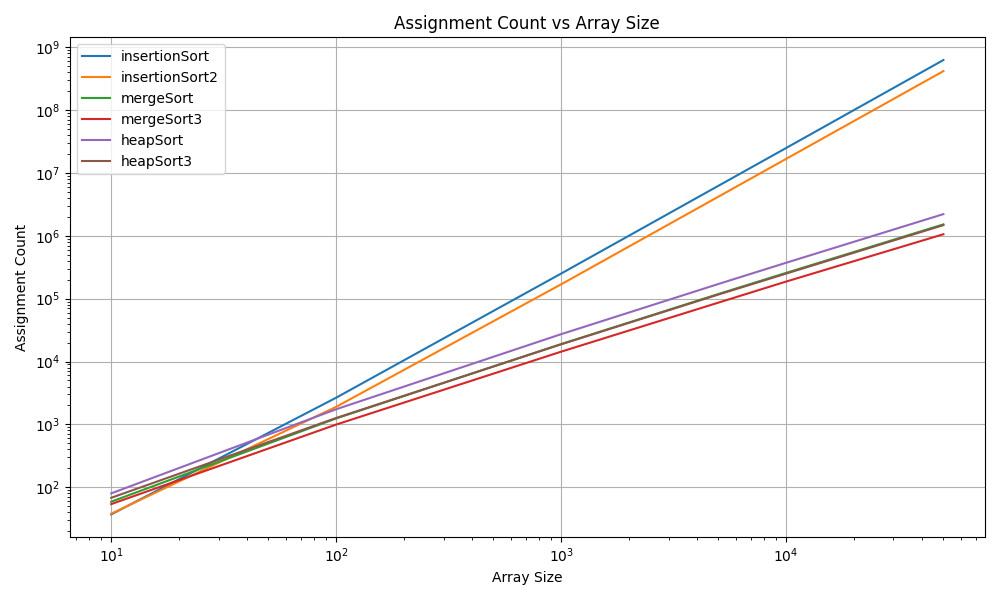
\includegraphics[width=0.95\linewidth]{Assignment plot.png}

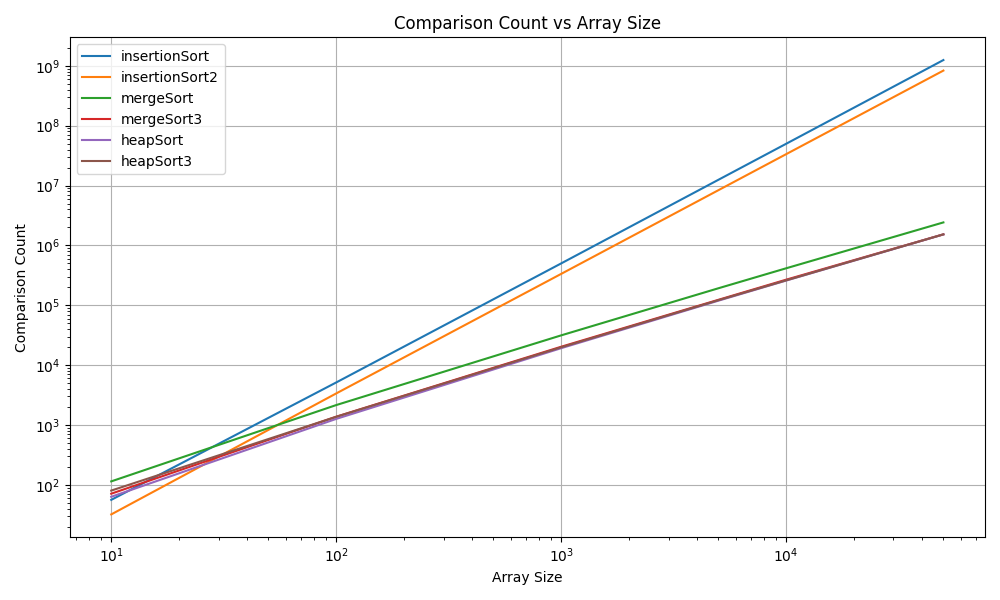
\includegraphics[width=0.95\linewidth]{Comparison plot.png}


Z tego powodu wykonałem kolejne testy na listach mniejszej wielkości, co pozwoliło na stworzenie wykresów bez skali logarytmicznej na których dużo lepiej widać różnicę we wzroście.

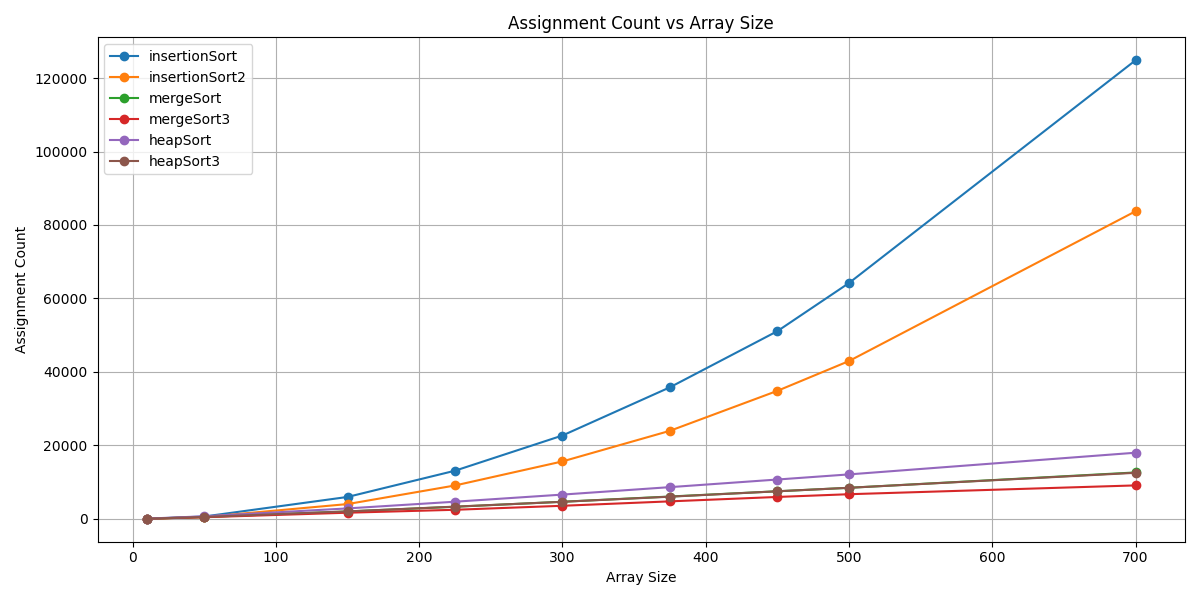
\includegraphics[width=0.95\linewidth]{Assignment plot small.png}

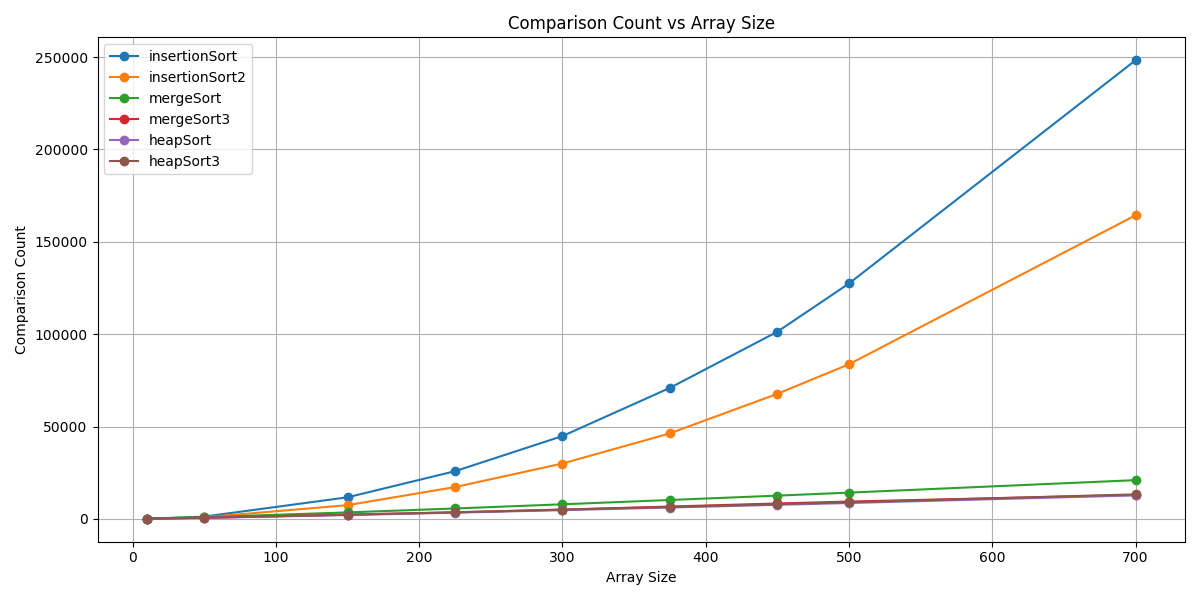
\includegraphics[width=0.95\linewidth]{Comparison plot small.png}

\section{Wnioski}

Algorytmy sortujące bardzo różnią się wydajnością między algorytmami \(O(n^2)\) a \(O(n\log{n}\) i używanie tych pierwszych jest dużo wolniejsze niż tych drugich, niewielka przewaga \(O(n^2)\) przy małych listach jest nieznacząca w większości przypadków dla krótkich czasów. Jedyne ich zastosowanie wydaje się być dla programów które muszą sortować ogromne ilości krótkich list.

Byłem też zaskoczony widoczną przewagą wydajności zmodyfikowanych algorytmów, choć ma ona sens - w przypadku merge i heap sorta intuicja podpowiada że powinna ona wzrosnąć około \(\ \log_2{3}\approx1.585\) krotnie, co rzeczywiście widzimy (np. dla merge sort o długości 50000 iloraz ilości porównań to \( \frac{2420827}{1529524}\approx1,582\)).

\end{document}
